% Editable native composition from verified original IDE photographs.
\par
\begin{figure}[htbp]
  \centering
  \sbox0{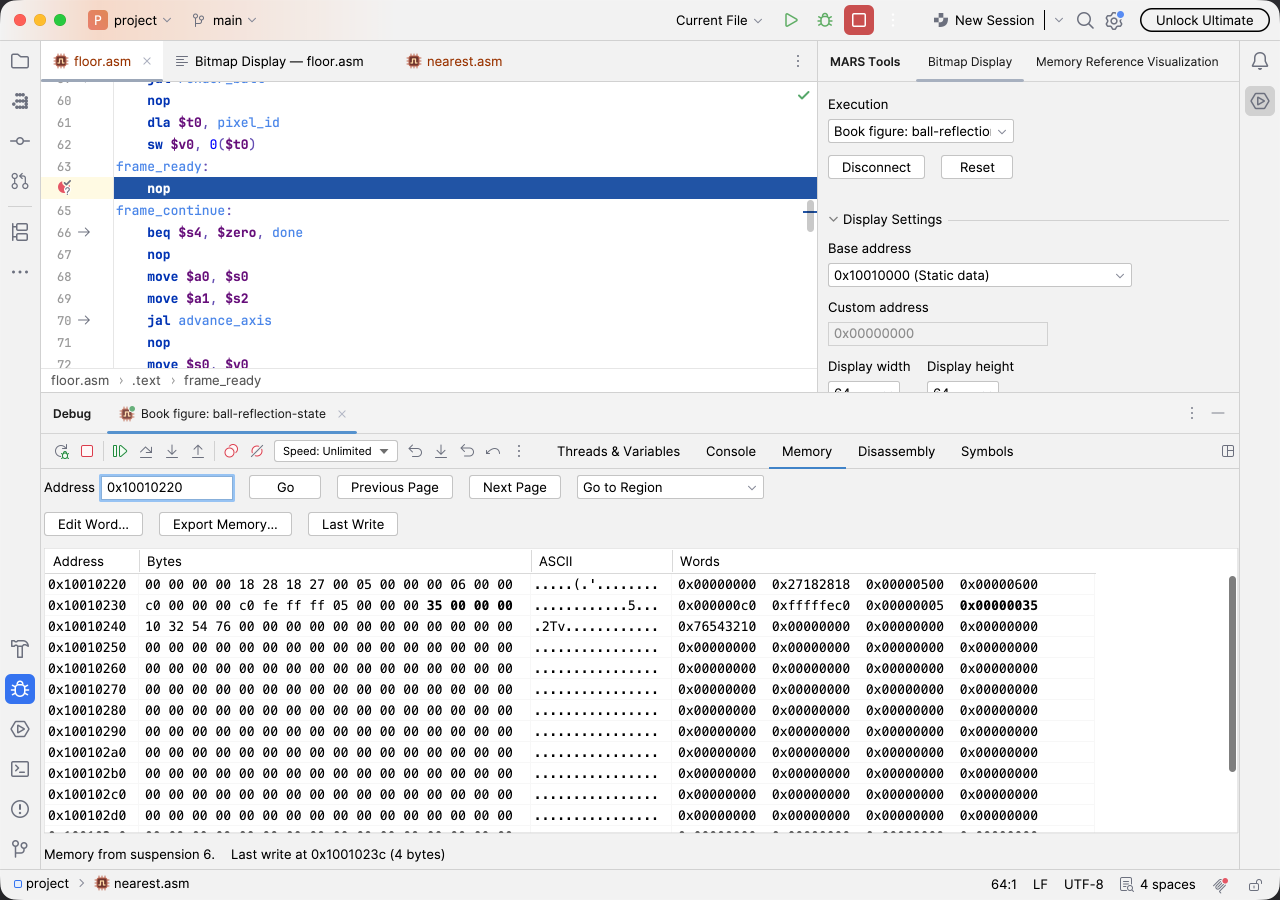
\includegraphics[artifact]{packages/012-fixed-point-ball/captures/f03-reflection/state.png}}
  \sbox2{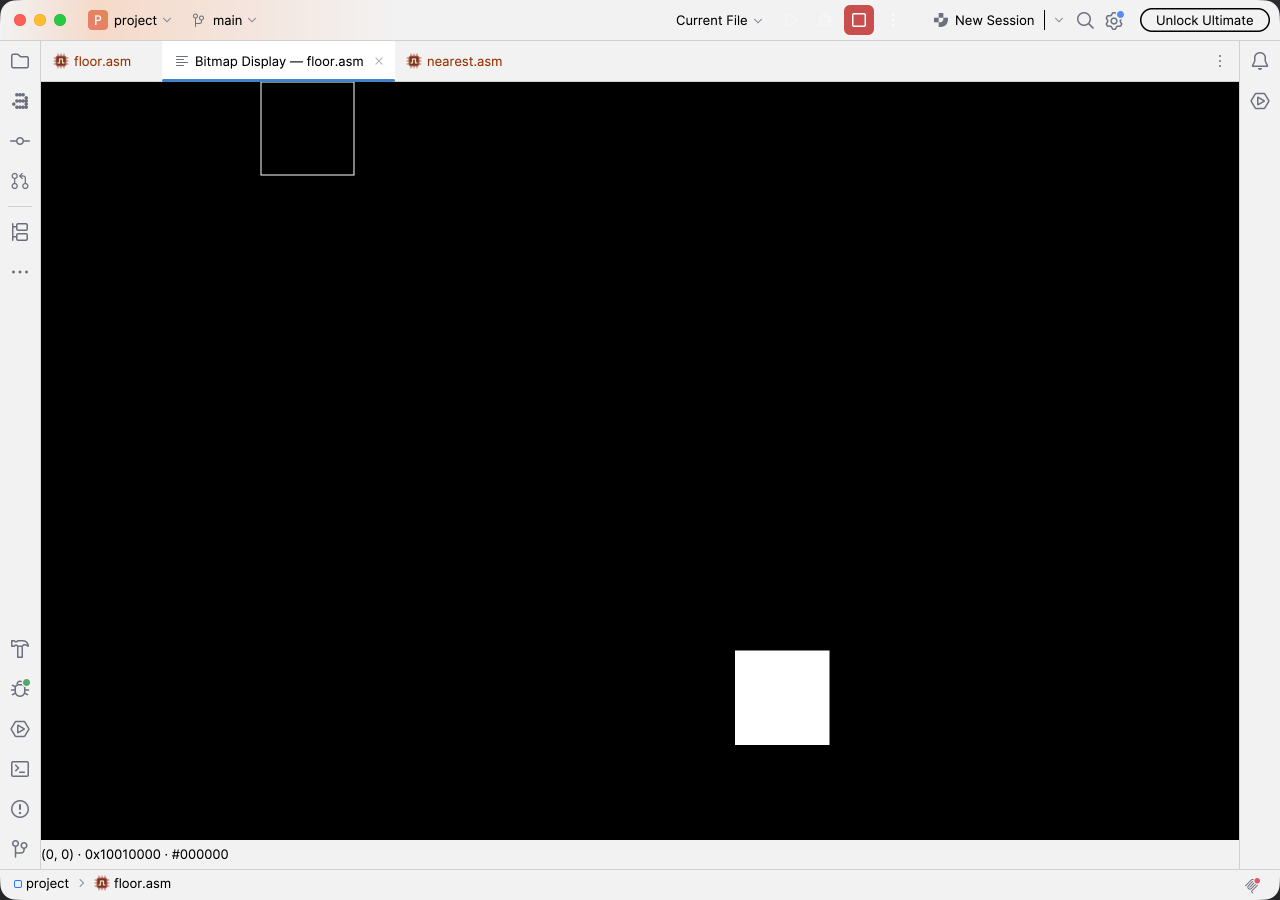
\includegraphics[artifact]{packages/012-fixed-point-ball/captures/f03-reflection/bitmap.png}}
  \edef\MARSballreflectionsourceLeft{\the\dimexpr0.036718750\wd0\relax}
  \edef\MARSballreflectionsourceBottom{\the\dimexpr0.774444444\ht0\relax}
  \edef\MARSballreflectionsourceRight{\the\dimexpr0.713281250\wd0\relax}
  \edef\MARSballreflectionsourceTop{\the\dimexpr0.147777778\ht0\relax}
  \edef\MARSballreflectionstateLeft{\the\dimexpr0.034375000\wd0\relax}
  \edef\MARSballreflectionstateBottom{\the\dimexpr0.311111111\ht0\relax}
  \edef\MARSballreflectionstateRight{\the\dimexpr0.584375000\wd0\relax}
  \edef\MARSballreflectionstateTop{\the\dimexpr0.608888889\ht0\relax}
  \edef\MARSballreflectionbitmapLeft{\the\dimexpr0.203906250\wd2\relax}
  \edef\MARSballreflectionbitmapBottom{\the\dimexpr0.066666667\ht2\relax}
  \edef\MARSballreflectionbitmapRight{\the\dimexpr0.203906250\wd2\relax}
  \edef\MARSballreflectionbitmapTop{\the\dimexpr0.091111111\ht2\relax}
  \begin{tikzpicture}[alt={Three annotated details after the first vertical reflection in floor mode. Tick five publishes raw x 1280, y 1536, horizontal velocity 192 and vertical velocity minus 320. The complete eight-by-eight frame has one white cell at column five, row six, ID fifty-three. The model reflects the tentative y coordinate eight pixels around the seven-pixel wall to six pixels.}]
    \node[anchor=north west,inner sep=0,font=\small\bfseries] (source-title) at (6mm,0) {Next instruction};
    \node[anchor=north west,inner sep=0] (source) at ([yshift=-1mm]source-title.south west) {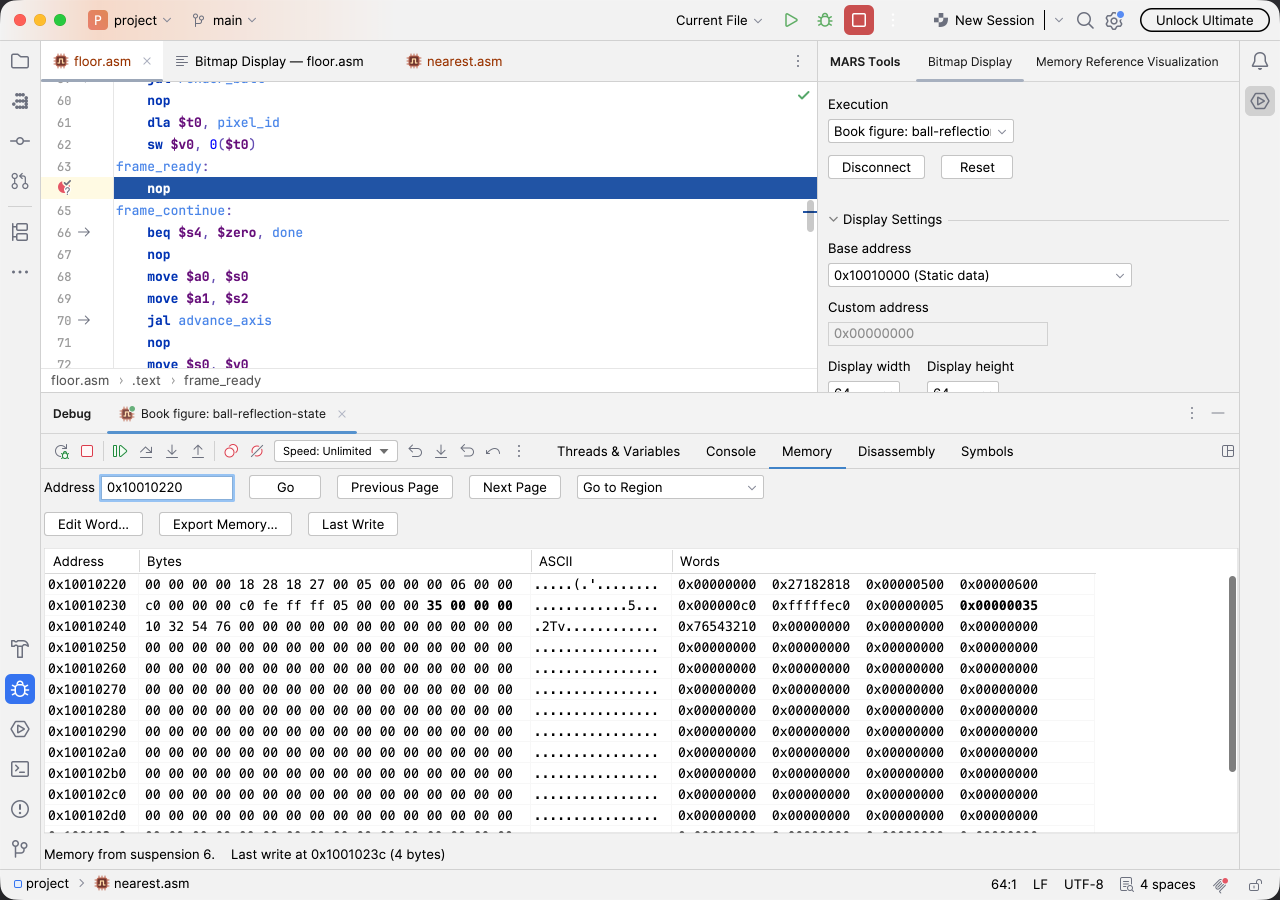
\includegraphics[width=0.58\linewidth,artifact,trim={\MARSballreflectionsourceLeft{} \MARSballreflectionsourceBottom{} \MARSballreflectionsourceRight{} \MARSballreflectionsourceTop{}},clip]{packages/012-fixed-point-ball/captures/f03-reflection/state.png}};
    \begin{scope}[shift={(source.south west)},x={($(source.south east)-(source.south west)$)},y={($(source.north west)-(source.south west)$)}]
      \draw[black,line width=0.7pt] (0.215625000,0.057142857) rectangle (0.384375000,0.371428571);
      \node[draw=black,fill=white,circle,inner sep=1.5pt,font=\footnotesize] at ($(0.215625000,0.371428571)+(-3mm,0)$) {1};
    \end{scope}
    \node[anchor=north west,inner sep=0,font=\small\bfseries] (state-title) at ([yshift=-3mm]source.south west) {Published raw state in little-endian words};
    \node[anchor=north west,inner sep=0] (state) at ([yshift=-1mm]state-title.south west) {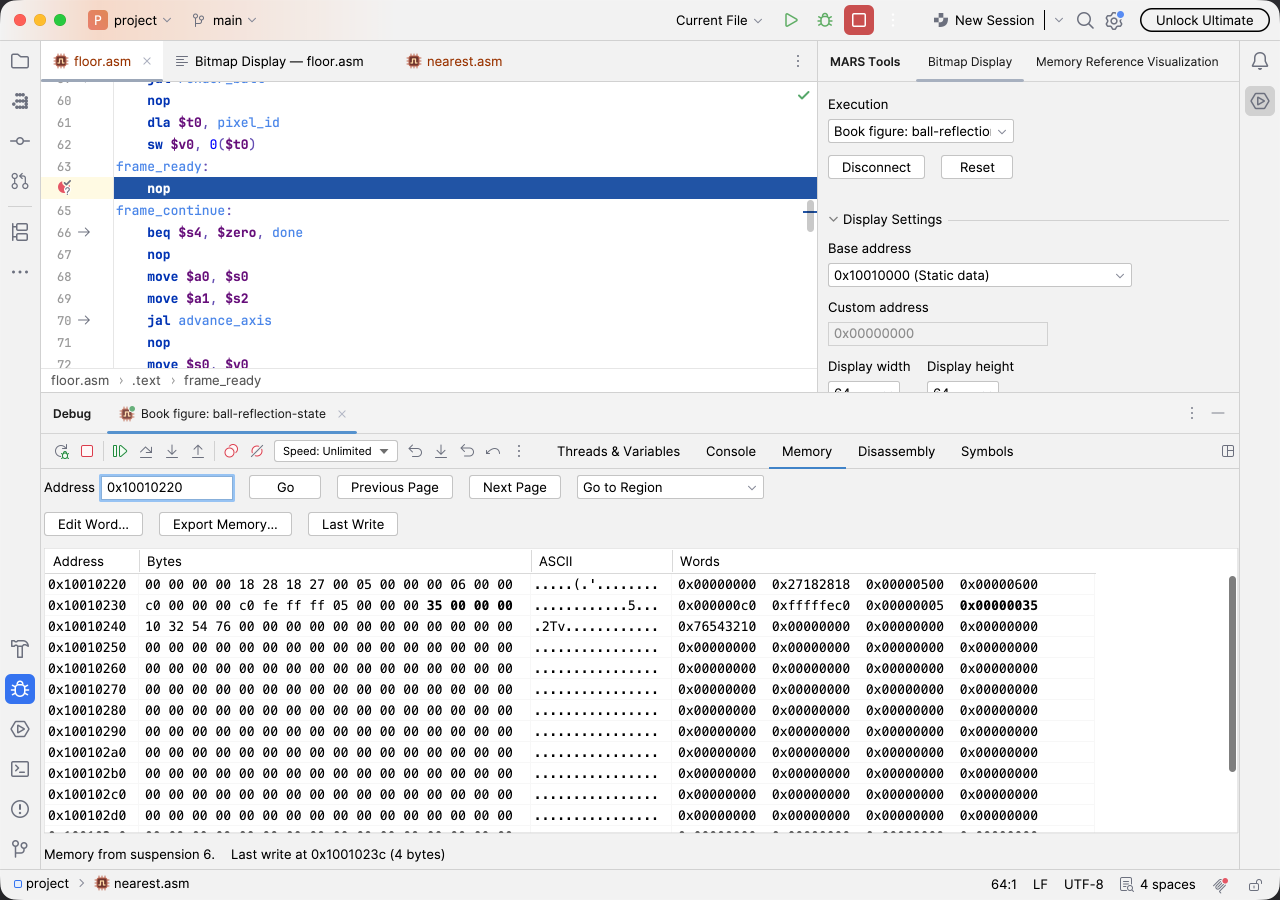
\includegraphics[width=0.85\linewidth,artifact,trim={\MARSballreflectionstateLeft{} \MARSballreflectionstateBottom{} \MARSballreflectionstateRight{} \MARSballreflectionstateTop{}},clip]{packages/012-fixed-point-ball/captures/f03-reflection/state.png}};
    \begin{scope}[shift={(state.south west)},x={($(state.south east)-(state.south west)$)},y={($(state.north west)-(state.south west)$)}]
      \draw[black,line width=0.7pt] (0.194672131,0.055555556) rectangle (0.997950820,0.638888889);
      \node[draw=black,fill=white,circle,inner sep=1.5pt,font=\footnotesize] at ($(0,0.638888889)+(-3mm,0)$) {2};
    \end{scope}
    \node[anchor=north west,inner sep=0,font=\small\bfseries] (bitmap-title) at ([yshift=-3mm]state.south west) {Complete eight-by-eight frame};
    \node[anchor=north west,inner sep=0] (bitmap) at ([yshift=-1mm]bitmap-title.south west) {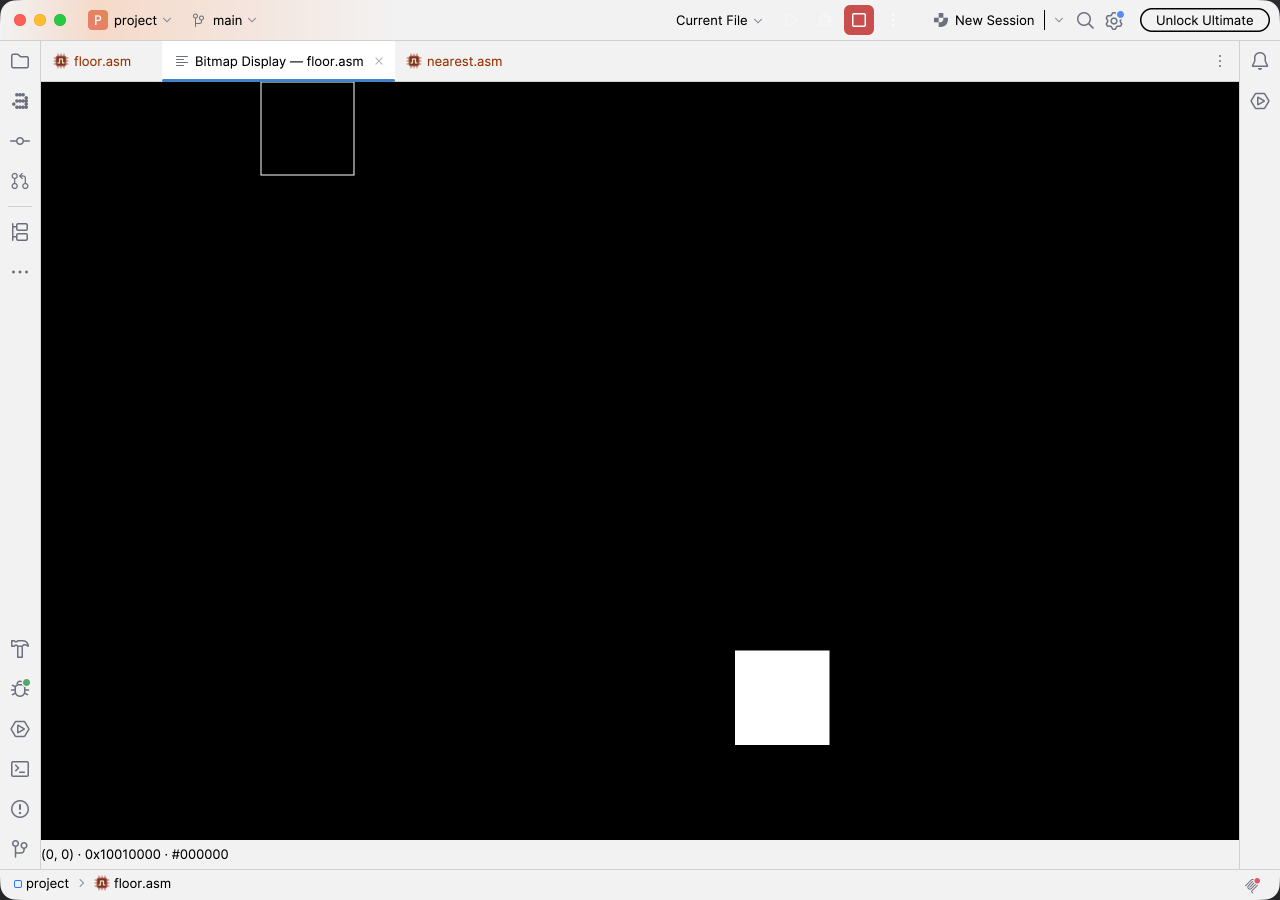
\includegraphics[width=0.28\linewidth,artifact,trim={\MARSballreflectionbitmapLeft{} \MARSballreflectionbitmapBottom{} \MARSballreflectionbitmapRight{} \MARSballreflectionbitmapTop{}},clip]{packages/012-fixed-point-ball/captures/f03-reflection/bitmap.png}};
    \begin{scope}[shift={(bitmap.south west)},x={($(bitmap.south east)-(bitmap.south west)$)},y={($(bitmap.north west)-(bitmap.south west)$)}]
      \draw[black,line width=0.7pt] (0.000000000,0.000000000) rectangle (1.000000000,1.000000000);
      \node[draw=black,fill=white,circle,inner sep=1.5pt,font=\footnotesize] at ($(0.000000000,1.000000000)+(-3mm,0)$) {3};
      \foreach \c in {0,...,7} {\node[anchor=north,font=\scriptsize,inner sep=0] at ({(\c+0.5)/8},-0.035) {\c}; \node[anchor=east,font=\scriptsize,inner sep=0] at (-0.025,{1-(\c+0.5)/8}) {\c};}
      \node[anchor=north,font=\scriptsize,inner sep=0] at (0.5,-0.11) {$x$}; \node[anchor=east,font=\scriptsize,inner sep=0] at (-0.10,0.5) {$y$};
    \end{scope}
  \end{tikzpicture}
  \par\smallskip
  \begin{minipage}{\linewidth}
    \small
    \begin{enumerate}
      \setlength{\itemsep}{2pt}
            \setlength{\parsep}{0pt}
      \item The native condition \texttt{\$s5 == 5} selects the sixth \texttt{frame\_ready} publication. It follows five complete motion updates; the initial publication was tick 0. The next marker instruction has not yet executed.
      \item The raw coordinates are now $1280/256=5$ and $1536/256=6$. The second line contains horizontal velocity 192, vertical bytes \texttt{c0 fe ff ff}, tick 5 and ID \texttt{0x35}=53. Interpreted as a signed word, \texttt{0xfffffec0} is $-320$, or $-1.25$ pixels per step. Previously $y=1728$ and $v_y=320$ gave tentative raw 2048, one pixel beyond the wall at 1792. Reflection gives $2\cdot1792-2048=1536$ and reverses the velocity. It preserves the overshoot rather than clamping to the wall.
      \item Floor displays $(5,6)$, giving $8\cdot6+5=53$. Rows increase downward, so the negative vertical velocity means upward motion. The frame contains the newly selected white cell and clears the old one; the entire 64-word frame is checked. The thin $(0,0)$ outline remains a selection marker.
    \end{enumerate}
  \end{minipage}
  \caption{At tick five, the vertical overshoot has been reflected and the ball is traveling upward.}
  \label{capture:012-fixed-point-ball-f03-reflection}
  \label{ball-f03-reflection}
\end{figure}
\par
